\subsection{Output Modalities}

In order to obtain an immersive experience, these are the most commonly available hardware setups (see figure \ref{FIG-HMD-CLUSTER-CAVE}):

\begin{description}
	\item[Head-Mounted Display (HMD)] --
	  Head-mounting displays are glass-shaped devices, projecting a pair of stereo-transformed images
	  to the user's retinas.
	  They often feature gyroscopes or similar apparatus to measure head orientation and tilt.
	  There are two kinds of HMDs: opaque and translucid --
	  in the former the images are projected on small opaque screens;
	  in the latter the projected surface is translucid, allowing blending of real and virtual worlds.
	  Translucid HMDs are best suited for Augmented Reality.
	  
		Using an HMD has the benefit of sticking to the user's head and detecting head orientation.
		On the other hand each HMD serves one single user and has limited resolution.
		Additionally, most users report suffering from fatigue after long periods of
		usage \cite{VREDUC}.
		Opaque HMDs have the additional downside of users being unable to see the real world, 
		which can be confusing as noted by \cite{VANDERPOL}.
			
	\item[Cave Automatic Virtual Environment (CAVE)] --
	  A CAVE is an immersive virtual reality environment where projectors are directed to four,
	  five or all the six walls of a room-sized cube.
	  
		It shares the benefit of enclosing the user's viewing area with HMDs and has better resolution.
		The downside is the small number of simultaneous users who can experience the CAVE at the same time
		and the inability to set up some tracking systems due to space constraints.
	
	\item[Large Screen Display (LSD)] --
	  An LSD is a large surface, usually planar, where a high resolution image is projected to.
	  The bigger, higher resolution LSDs require a grid of projectors to project parts of the overall resulting image.
	  In this case the projectors get their information from several computers working in a cluster.
	  
	  The whole image projection is responsibility of a cluster of projectors set up in a wall.
	  Each projector renders part of the surface and the border between projections is ideally minimal.
	  Each projector is controlled by an independent computer.
	  
		Its size and resolution depend entirely on the setup, but oftentimes a wall offers higher resolutions
		(depending on the number of projectors in the grid and each projector's resolution)
		than the remaining discussed hardware setups.
		Due to the large surface of the wall, several users may be served as once.
		Another benefit is the freedom of movement given to users due to users not carrying wires \cite{INTTABLE}.
		The downside is users having to face the wall to experience the image entirely.
\end{description}

\begin{figure}[!ht]
	\centering
	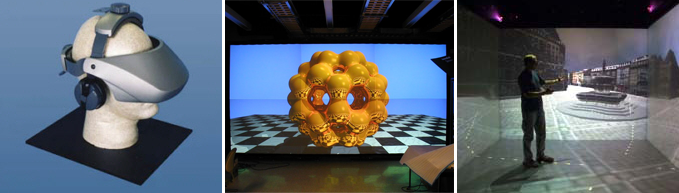
\includegraphics[width=12cm]{gfx/hmd-cluster-cave.png}
	\caption{HMD, Wall, CAVE}
	\label{FIG-HMD-CLUSTER-CAVE}
\end{figure}

Any of these setups is suitable for single user interaction.
In case of a reviewing session at which at least two participants are required,
CAVEs or LSDs are better suited, since they both offer a single solution for a small group of people.

Using a CAVEs or LSDs presents other challenges:
the computers responsible for the generation of the projectors' images must be synchronized,
the projectors color parameters calibrated and the viewport must be well cropped.
There are several systems capable of delivering high performance 3D graphics and
offering the features mentioned above.
Based on scene graphs there are two well established solutions:
OpenSceneGraph\cite{SITE-OSG} and OpenSG\cite{SITE-OPENSG}.
The framework on top of which our system was build runs on OpenSG.